% !TEX root = ../proposal.tex


\subsection{Management structure and procedures}
\label{sec:management}

% - Describe the organisational structure and the decision-making (
%   including a list of milestones (table 3.2a))
%
% - Explain why the organisational structure and decision-making
%   mechanisms are appropriate to the complexity and scale of the
%   project.
%
% - Describe, where relevant, how effective innovation management will
%   be addressed in the management structure and work plan.
%   
%   Innovation management is a process which requires an understanding
%   of both market and technical problems, with a goal of successfully
%   implementing appropriate creative ideas. A new or improved product,
%   service or process is its typical output. It also allows a
%   consortium to respond to an external or internal opportunity.
%
% - Describe any critical risks, relating to project implementation,
%   that the stated project's objectives may not be achieved. Detail any
%   risk mitigation measures. Please provide a table with critical risks
%   identified and mitigating actions (table 3.2b)

\subsubsection{Management Structure}

\begin{wrapfigure}{r}{0.4\textwidth}%
    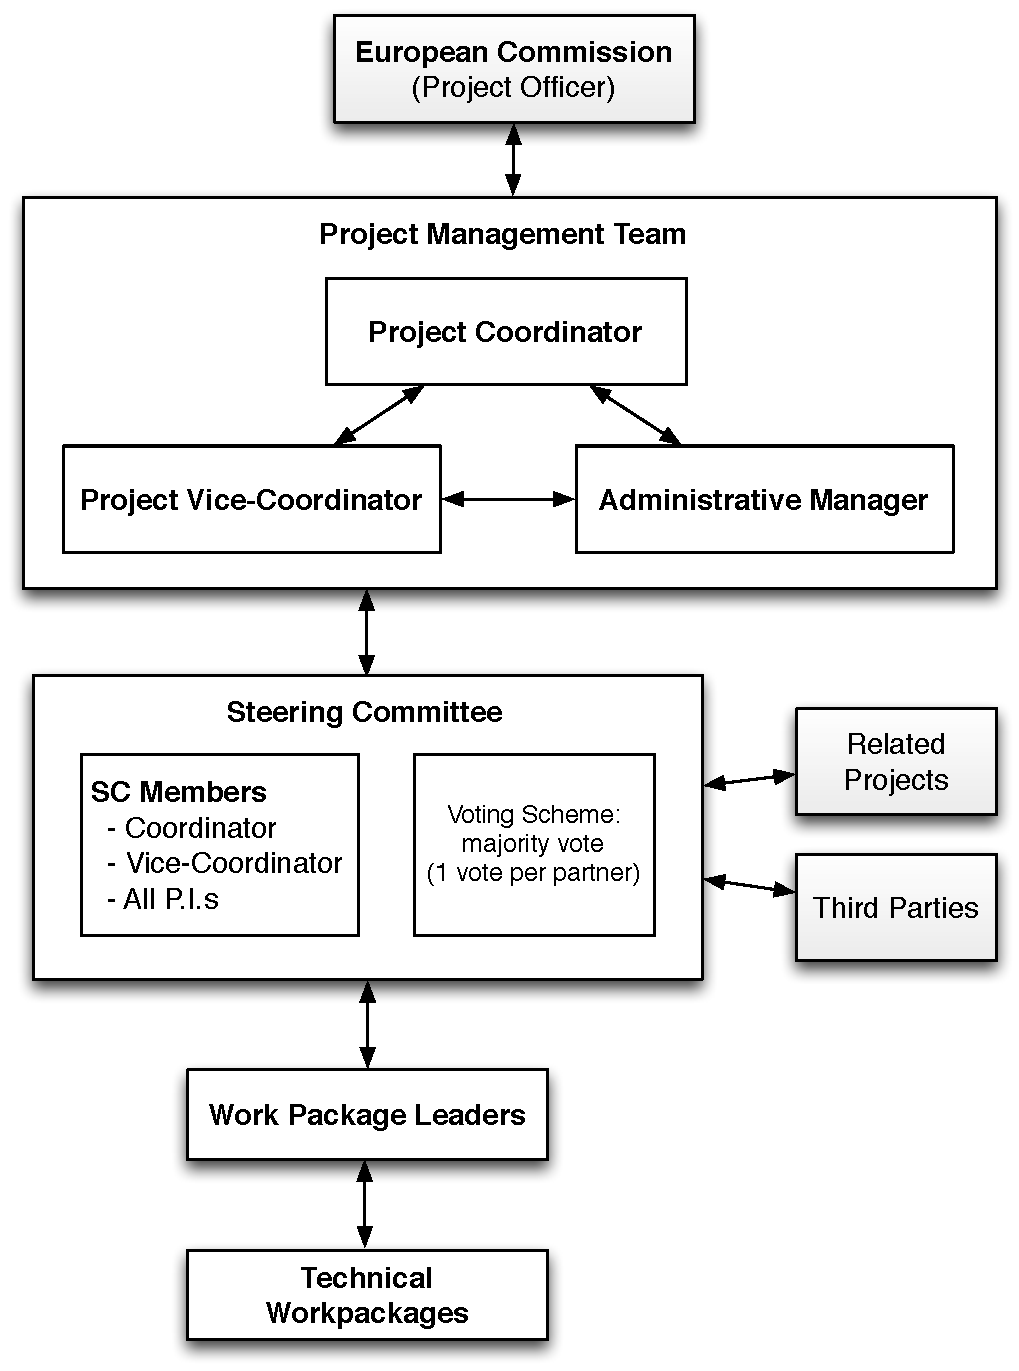
\includegraphics[width=0.4\textwidth]{pics/mngt2}
    \caption{Management scheme for \Project.}
    \label{fig:management}
\end{wrapfigure}

The project management team will
implement clear management processes and promote a qualitative and
dynamic management of all aspects of the project.

The {\em Project Coordinator}, \Coordinator{} from \COORD, has
extensive experience in organizing and supervising international
research projects. He will be
responsible for the overall project strategy, ensuring that all
parties within the consortium know exactly what is expected from them,
as described in the individual work packages.  \Coordinator{} will be
responsible for ensuring that all objectives are met and that all
costs and milestones are in line with the budgets and the provided
Gantt chart. Any deviation will be immediately communicated to the
consortium members and the EC Project Officer.

\Project{} will use the {\em Steering Committee} as a key element of
the project management structure for decision making. It consists of
all PIs, and the Coordinator. The Coordinator will take care of the management of the
project and will ensure the execution of the contract.

\Project{} will be managed and monitored in a clear and effective
manner. It will be organized as depicted in the diagram shown in
Figure~\ref{fig:management}.  In the following, we describe the
individual management structures.



\vspace{3mm}
{\bf The Project Coordinator}


As the Coordinator, \Coordinator{} is the single point of contact
between the European Commission and the consortium.  In this function,
the Coordinator shall:
\begin{denseItemize}
\item Sign the contract with the European Commission
\item Ensure access to the contract by the other contractors
\item Ensure the communication between the consortium and Commission
\item Receive and distribute the EC contribution
\item Collect the cost statements from all contractors for submission
  to the European Commission
\item Prepare, with the support of the consortium, the reports and
  project documents required by the EC %%European Commission
\item Ensure prompt delivery of hardware, software and data
  identified in the contract or requested by the European Commission
  for reviews, including the results of the financial audits prepared
  by independent auditors
\end{denseItemize}

\Coordinator{} will monitor the scientific progress at the
individual partners' sites. He is authorized to execute the project management. Further, he will be accountable to
the project Steering Committee, will be responsible for the
preparation of the Steering Committee meetings and for chairing them.

The following activities belong to the responsibilities of the project
management:
\begin{denseItemize}
  \item The overall legal, contractual, ethical and administrative
  management of the project
  \item Financial management for the Coordinator
  \item Cost calculations for personnel (contracts, time-sheets, \etc), travel, meetings, and equipment (amortization, monitoring of resources)
  \item Juridical advice and administrative advice
  \item Overseeing the promotion of gender equality in the project
  \item Contact management (consortium and EU Project Officer)
  \item Preparing, updating and managing the consortium agreement
    between the participants
  \item Preparing project documents for the Coordinator including
    contracts, meeting minutes, \etc
  \item Decisions on documentation standards
  \item Project Manual for the consortium
  \item Monitoring of important dates and deadlines
  \item Day-to-day management activities
  \item Organization of meetings
  \item Implementation of decisions made by the Coordinator and the
    Steering Committee
  \item Obtaining audit certificates (as and when required) by each of
    the Contractors
  \item Collection of financial reports
  \item Preparation and coordination of project documents such as
    progress and final reports, including Form C, management reports, technical reports, final report, and publishable summary
  \item Supervision of project objectives and timeliness of the work plan
  \item Monitoring and illustration of the project status and data of the partners
  \item Maintaining a project calendar
  \item Management of letters, reminders, transactions
  \item Support the negotiations for late or low-quality activities
\end{denseItemize}


%\vspace{3mm}
{\bf Steering Committee}
\label{sec:mngt:ga}

The \Project{} project has a clear structure and a well-defined
management scheme (see Figure~\ref{fig:management}) with the Steering
Committee as its key decision making instrument.  It is the core
organizational and decision-making body and has the obligation to
ensure that the consortium functions properly.  It will be responsible
for the successful completion of the project and the exploitation of
its results.  It will be chaired by the appointed Project
Coordinator. Further core members of the Steering Committee will
all PIs.  Decisions regarding the project will be made by vote with
each partner having a single vote. A majority of voting members is
required to conduct a meeting (quorum). A simple majority is required
to make formal decisions.  In cases of a tie, the Project Coordinator
will have a casting vote.  Non-voting members and external experts may
be invited by the Chair.

The Steering Committee will normally meet every six months and it
represents the consortium in all related affairs. The duties include,
but are not limited to:
\begin{denseItemize}
\item All budget-related matters
\item The structure and restructuring of the work packages
\item The alteration of the consortium agreement
\item The premature completion / termination of the project
\item Preparation of all documents (financial, reporting, audit, \etc)
\item Management of knowledge
\item Communication between the consortium and the Commission
\item Communication between the consortium and third parties
\item Publicity
\item Establishment and overview of intellectual property procedures
\item Preparation of detailed work plan
\item Steering of the consortium
\end{denseItemize}


\vspace{3mm}
{\bf The Work Package Leaders}

The \Project{} partners will contribute a wide variety of relevant and
sometimes exclusive knowledge, expertise and experience. To ensure the
optimal use of this expertise and to maximize fertile interaction
between partners, work is divided into work packages (WP) each of them
under the responsibility of a WP leader from each of the
partners. Each WP will ultimately be the responsibility of the WP
leader. The WP leaders are responsible for keeping the time schedule
and the appropriate implementation related to their WP. It is also
within their duties to make the necessary contacts with leaders of
other WPs, when their activities depend on the other person's
work. The \Project{} partners will always be informed as to the state
of affairs within every WP.

\vspace{3mm}
{\bf List of Milestones}

The six project milestones described in Section~\ref{sec:milestones} represent a set of quantitative measures for the management to verify the progress of the project. Table~\ref{tab:milestones} on Page~\pageref{tab:milestones} lists the milestones and means of verification.  The time-lines for the milestones and deliverables are presented in the Gantt chart in Figure~\ref{fig:gantt} on Page~\pageref{fig:gantt}.


\subsubsection{Key Project Meetings}
\label{sec:keymeetings}

The Steering Committee will meet at the start of the project and at
six-month intervals. The meetings will normally be scheduled to
rotate between the contractors home base.

The Coordinator will organize these meeting as well as the kick-off
meeting with all partners and the Commission's representative.
The purpose of the project \textbf{kick-off meeting} is to ensure an effective
beginning of the work by detecting and preventing possible problems in
the very beginning such as, for example, delays in the personnel
hiring procedures or device ordering.

%\clearpage
Besides the at least eight \textbf{meetings of the Steering Committee}
throughout the project life-cycle, there will be four
\textbf{integration and testing weeks} to boost the integration
efforts and to perform tests of the overall system. The integration
meetings are scheduled for
\begin{center}
\begin{tabular}{|l|l|}
\hline
\highlightCell Integration and Evaluation Meeting No. & \highlightCell Tentative Schedule \\ \hline\hline
1 (main focus on integration) & M17\\ \hline
2 (main focus on integration and evaluation) & M24\\ \hline
3 (main focus on integration and evaluation) & M41\\ \hline
4 (evaluation) & M48\\ \hline
\end{tabular}
\end{center}

In addition to the above mentioned project meetings, there will be
four \textbf{review meetings} for the project. Here, we follow a time
schedule for EU projects with a duration of 48 months. This results in
four review meetings as shown in the table below.
\begin{center}
\begin{tabular}{|c|l|}
\hline
\highlightCell Review No. & \highlightCell Reviewing Period \\ \hline\hline
1 & M1 -- M12\\ \hline
2 & M13 -- M24\\ \hline
3 & M25 -- M36\\ \hline
4 & M37 -- M48\\ \hline
\end{tabular}
\end{center}



\subsubsection{Management Procedure Tools}

The Coordinator will establish the following
management procedure tools:
\begin{denseItemize}

\item {\bf Project Handbook}: The Coordinator will set up an
  Implementation Strategy, including a the draft of a Project Handbook
  for the purpose of managing information flow, timescales scheduling
  and finance planning as well as best project quality assurance and
  project documentation. This project handbook will be updated as
  appropriate throughout the duration of the project.

\item {\bf Internal assessment}: The Coordinator will
  closely follow and control the progress of the project and the work
  done by each partner.  If the results of this assessment is critical
  or inappropriate, the Coordinator will approach the partner and try
  to help eliminating the problems. If this is not successful, the
  result will be transmitted to the Steering Committee to take
  appropriate actions.

\item {\bf The collaborative platform (Intranet)}: The collaborative
  platform is an Internet-based secured collaborative
  web-site/repository where all project partners can share and
  exchange information. This platform is intended to foster
  collaboration between all partners at all levels: consortium, WP leaders,
  Steering Committee, Coordinator, Project Officer, \etc. Its
  functions include scientific, administrative and financial
  information exchange and archiving. 

\item {\bf Project management software}: The project will use as
  knowledge management software application. The software will ease the financial and technical
  controlling and a constant follow up of the project with key
  performance indicators for an always open project supervision. It
  provides an in-depth view to optimize the work-flow and resource
  allocation in the project.
\end{denseItemize}



\subsubsection{Risks and other Critical Factors}
\label{sec:management:risks_crit_fac}

The consortium will identify the factors that are critical to the
final success of the project and control these factors. For this
purpose, the consortium will define methods and procedures to
identify, assess, monitor and control areas of risk. The challenge
underlying the project has been carefully analyzed. A table of risks
and risk mitigation measures has been included with each {\em work
  package description}. Here we outline project-level risks and our
contingency plans.

%\clearpage

\begin{riskslabeled}{The Cohesiveness of the Consortium}
%%%%%%%%%%%%%%%%%%%%%%%%%%%%%%%%%%%%%%%%%%%%%%%%%%%%%%%%%%%
\item Consortium has no harmony
\putright{ {\em Impact: high, Risk: very low}}

{\em Evaluation:} The partners in the consortium have been carefully
selected, also based on experience with prior collaborations. Multiple
partners already worked together in the EU project V-Charge and other projects. Problems with respect to harmony in the
consortium may arise when the plan of activities is not fully
understood by all participants or when personal incompatibilities
arise during the work. This is very unlikely the case in this proposal
however, since all partners have been intensively involved during the
write-up stage and, in particular, when it came to authoring the parts
for which they bring in their expertise. Thus, all partners are very
well aware of what they committed to.

{\em Resolution:} Previous experiences within the partners have been
very positive and should be maintained at consortium level. In the
very unlikely case of serious conflicts, the conflict resolution
strategies of Section~\ref{sec:confl_mng} will be brought to bear.


%%%%%%%%%%%%%%%%%%%%%%%%%%%%%%%%%%%%%%%%%%%%%%%%%%%%%%%%%%%
\item Poor quality of deliverables
\putright{ {\em Impact: high, Risk: low}}

{\em Resolution:} The Coordinator will monitor the deliverables and
will immediately react in case of low quality. Please note that the
members of the \Project{} consortium are all experienced with
participating in and managing of European research projects, and thus
know the high quality that is expected of the deliverables.



%%%%%%%%%%%%%%%%%%%%%%%%%%%%%%%%%%%%%%%%%%%%%%%%%%%%%%%%%%%
\item Delay in meeting the deadlines
\putright{ {\em Impact: medium, Risk: medium}}

{\em Resolution:} The progress of the project will be assessed at
frequent intervals to predict possible delays and to act
accordingly. The spiral development models allow us to significantly
reduce the risk of delay for components on which others depend.  The
intermediate deliverables developed in the first phase of the spiral
serve as prototypes of software components with limited functionality
will be delivered to the consortium. This also allows us to react
timely in case of upcoming problems and resolve the issues
\emph{before} any critical situation arises. By also controlling if
all partners have successfully started their RTD activities (Milestone
MS1 at M4), the risk of delays in the development is further reduced.
\end{riskslabeled}

%\vspace{5mm}

\begin{riskslabeled}{Technology-Related Problems}

%%%%%%%%%%%%%%%%%%%%%%%%%%%%%%%%%%%%%%%%%%%%%%%%%%%%%%%%%%%
\item The complexity of integration compromises system performance
\putright{ {\em Impact: high, Risk: low}}


{\em Resolution:} Experience of developers is essential to contain this risk. To this end great attention has been devoted during project preparation to the design of clear interfaces between work packages. Any remaining unmodeled interdependencies are expected to be approachable in an effective and timely manner, thanks to the use of the spiral development approach. Furthermore, all members of the
consortium have great experience in large research projects and in the
integration of large and complex systems. Therefore, the likelihood
that such problems will compromise the project is low.


%%%%%%%%%%%%%%%%%%%%%%%%%%%%%%%%%%%%%%%%%%%%%%%%%%%%%%%%%%%
\item Risk plans prepared at the end of each work package may be
  missing important points \putright{ {\em Impact: low, Risk: low}}

{\em Resolution:} To assure that the work packages will be executed
correctly, assessment of the risk plans for each of the work packages
will be made again before they start of the project and updated throughout.

\end{riskslabeled}

\vspace{5mm}


\begin{riskslabeled}{Other Risks}

% %%%%%%%%%%%%%%%%%%%%%%%%%%%%%%%%%%%%%%%%%%%%%%%%%%%%%%%%%%%
 \item Difficulties in handling IPR \putright{ {\em Impact: high, Risk: very low}}

{\em Resolution:} To lower this risk, a consortium agreement will be
 signed before the start of the project.  Furthermore, all partners
 agreed already now on an IPR strategy. The key decisions that are
 formulated in this strategy are summarized in Section~\ref{sec:iprhandling} on
 page~\pageref{sec:iprhandling}. Thus, IPR related issues should not affect the
 developments within the project.
 \end{riskslabeled}




\subsubsection{Conflict Management}
\label{sec:confl_mng}

Conflicts are part of everyday life and occur while working together
in international projects, also for reasons of different cultural
backgrounds. Therefore, possibilities that are available to reduce
conflict potentials will be pursued such as cooperative leadership in
the project and the different working teams. Communication between
consortium members will be facilitated in meetings, telephone and web
conferences so that they get to know each other intensively and
appreciate cultural differences. All project data will be documented
and made available on the shared workspace. If conflicts arise, they
will be firstly internally (by voting) and if necessary externally
solved via mediation techniques (involving a neutral person). In case
of persisting conflicts, the issue will be discussed with the Project
Coordinator who is entitled to overrule all prior voting or moderated
results. In this way, it can be guaranteed that the project is able to
take decisions and function at any time.

Pragmatic negotiation will be the basis for the consortium conflict
resolution approach. Typical conflicts, which can arise in the
project, can be due to a lack of productivity and/or quality, missed
deadlines, different languages and personality or cultural
differences. It will be the responsibility of the Coordinator to identify these
conflicts at an early stage and take steps to talk to the involved
parties to quickly resolve the conflict.  {\em Negotiations} and
decisions taken by consensus will be the main tools to resolve
conflicts.

In case a conflict should arise between the parties, a mediation
procedure shall be started within the consortium. The Coordinator (if
not part of the conflict; should this be the case a neutral
participant of the project will provide to substitute the Coordinator)
will proceed with the following steps:
\begin{denseItemize}
\item Meeting with the conflict parties within one month after being
  officially informed by letter
\item Mediation through an external expert
\item Vote by the Steering Committee
\item European Commission consultation
\item If no other solution is possible devolution to an external court
  of arbitration
\end{denseItemize}

All decision-making procedures and conflict-resolution mechanisms will
be refined and detailed in the consortium agreement.

\subsubsection{Methods of Monitoring and Reporting Progress}

The Steering Committee is an experienced project management team and will
use different methods for monitoring in form of analyses. Each partner is requested to informally report on a
regular basis on progress and deployed resources. In addition to that,
any problems, expected delays, or other events that may impact the
developments in \Project{} have to be reported to the Coordinator as
soon possible.  The documentation standard will be provided by the
Coordinator. All information will be summarized and
distributed to the partners with remarks and countermeasures in case
of major deviations.

All partners will have the responsibility to report to the
Coordinator who has the responsibility to
collect and summarize the reports.  



\subsubsection{Communication Flow}
\label{sec:mngt:comm}
Ensuring a good communication among project partners and towards
outside entities represents an important key of success for the
project and a fundamental practice to manage the project at its best.

The establishment of a fast, reliable and easily accessible
communications infrastructure is vital to the proper operation of a
pan-European project. This can only be achieved through the intensive
use of electronic communications (\eg, email, web based exchanges, Twitter). A
project web-site will also be used to enable fast and efficient
exchanges of information. Thus, main communication channels are
\begin{denseItemize}
\item telephone calls and telephone conferences
\item email
\item web-based services such as internal discussion forums or chats
\item personal meetings
\end{denseItemize}

The internal communication includes physical meetings, starting with a
1-2 day kick-off meeting to guarantee in-depth knowledge exchange.  It
has been planned to have at least six-monthly of the Steering Committee during the project life cycle.  Meetings can also be
accompanied via telephone conferences to discuss project progress and
to take decisions. Also applied are the exchange of emails, letters,
\etc. The advantages of these tools lie in their
functions of allowing the sharing of documents, contact details, white
boards, discussion rooms, \etc. The management team will introduce
such a tool to increase transparency and trust among the project
partners.

The communication flow between \Project{} members will be implemented by:
\begin{denseItemize}
\item Periodic meetings of the Steering Committee
\item Individual working meetings of members of each WP
\item Phone and e-mail interchanges (day to day cooperative working infrastructure)
\end{denseItemize}

The Coordinator has the duty to communicate on a
systematic and frequent basis even if no problems are identified with
every WP leader during the life cycle of their WP to assure the smooth
flow of \Project{} project activities.

All ordinary messages related to a certain work package will be
communicated among all partners involved in that
work package. Nevertheless, any particularly important issues or problems
within the frame of a WP are going to be forwarded to the WP leader
and, if needed, to the Steering Committee.

The experience in running research projects, the good relationships,
and mutual knowledge of the partners as well as their previous
successful collaborations, almost ensures the prevention of problems
regarding communication and information flow within the \Project{} project.


\subsubsection{Statement of Quality}

The \Project{} consortium recognizes that a dedication to quality is
vital to our mission and is essential for delivering
consistent results. Therefore, the consortium agrees on developing a
Statement of Quality with regards to its work.


To achieve its mission, the \Project{} consortium will establish
quality assurance procedures. Underlying these procedures is a set of
principles, which inform the \Project{} Project quality
approach. These are:
\begin{denseItemize}
\item Document procedures, standards and control
\item Issue control for documents
\item Reporting procedures, frequency and format
\item Communication procedures
\item Corrective actions
\item Exception control
\item Conflict resolution
\item Meeting draft agenda
\item Format of meeting minutes
\item Tracking system for actions
\item Specific responsibilities within the project
\end{denseItemize}
\Project{} aims to assure the very highest quality in all the information and analysis it will provide.
All project partners are responsible for quality.  Quality is the
responsibility of every member of the consortium members' staff participating in
the \Project{} project. For the
successful accomplishment of this approach, there are clear lines of
responsibility and accountability for each WP and adequate support to
enable the staff to achieve their quality objectives.  

The \Project{} consortium recognizes that one important factor in assuring
quality is a constant re-examination of our work against the needs
of planned objectives. In this way, we can assure that we are
maintaining appropriate standards and also demonstrate accountability
to the Commission and the public in general of our work. The spiral life cycle approach supports this seamlessly.


\subsubsection{Evaluation Process}

The work progress of the \Project{} Project will be continuously
monitored and supervised by the management team.  In addition to that,
the evaluation meetings (see Section Key Project Meetings on
page~\pageref{sec:keymeetings}) will be carried out to evaluate the
work and progress of the project.

An internal peer review will be performed for each document
produced. Each WP leader will submit all the produced documents to an
appropriate expert internally, not
involved in the same WP, to check for the quality of the documents
produced.

A basis for measuring the quality of the conducted work are the
Measures of Success specified in the work packages descriptions
starting on Page~\pageref{wp1}. Furthermore, the publication of
achieved results in journals as well as European and international
conferences will be taken as a measure of success for the involved
universities and research teams.

Finally, as part of the evaluation process, we will apply a risk
management approach assessing risk in technical, operational and human
resources, the probability that they happen and the impact they will
have in the project. Risks will be reported in the management reports
as well as the actions to reduce the threats and to solve the
situations when these threats materialize.

\subsubsection{Consortium Agreement}

The first task of the Coordinator --  before the project starts -- will be the setup of a consortium
agreement between all the partners. This
procedure will begin immediately after receiving the project approval by the
commission. The consortium agreement will be agreed on and signed
before the beginning of the project.

The consortium agreement will cover the following aspects, as a
minimum:
\begin{denseItemize}
\item The internal organization and management of the consortium
\item Collective Responsibility of the partners
\item Intellectual property arrangements either generated during the
project or existing prior to or acquired in parallel with the project
\item Roles in the consortium
\item Financial viability and audits
\item Exploitation of the project results and commercial considerations
\item Settlement of internal disputes, change in consortium
membership, potential solutions to problems relating to the technical
implementation and solutions to potential financial problems
\end{denseItemize}


\subsubsection{Intellectual Property Handling}%

Intellectual property handling is specified in Section~\ref{sec:iprhandling}, see page~\pageref{sec:iprhandling}.

\subsubsection{Dissemination and Exploitation Activities}%

Details on dissemination and exploitation activities can be found in Section~\ref{sec:diss} on page~\pageref{sec:diss} and in Section~\ref{sec:expl} on page~\pageref{sec:expl}.

